\section{Implementación de bloques del sistema}
%%%%%%%%%%%%%%%%%%%%%%%%%%%%%%%%%%%%%%%%%%%%%%%%%%%%%%%%%%%%%%%%%%%%%%%%%%%5%%%%%%%%%%%%%%%%%%%%%%%%%%%%%%%%%%%%%%%%%%%%%%%%%%%%%
%por qué este algoritmo? cómo se hace? explicar la filosofía de conseguir una implementación y adaptarla a nuestro propósito, y que la realidad es que no hay muchos sistemas disponibles. La justificacion puede venir por dos ejes: complejidad del algoritmo, en uruguay no hay casi experiencia industrial en procesamiento de imagenes. por qué no se usó un detector de circulos? son cosas muy chicas y en realidad no son circulos perfectos. La explicación del algoritmo tiene que ser bien detallada. En qué lenguaje se programó, justificar herramientas (por qué opencv, por qué c++, etc.)
%%%%%%%%%%%%%%%%%%%%%%%%%%%%%%%%%%%%%%%%%%%%%%%%%%%%%%%%%%%%%%%%%%%%%%%%%%%%%%%%%%%%%%%%%%%%%%%%%%%%%%%%%%%%%%%%%%%%%%%%%%%%%%%%%%

%COMENTARIO: ACÁ SE ME OCURRE DE HACER UNA INTRODUCCIÓN A CADA BLOQUE DEL SISTEMA, JUSTIFICAR Y EXPLICAR MEDIO POR ARRIOBA Y EN LAS SIGUIENTES SECCIONES EXPLICAR LOS DETALLES MÁS TÉCNICOS DE CADA BLOQUE.


\begin{figure}[H]
\begin{center}
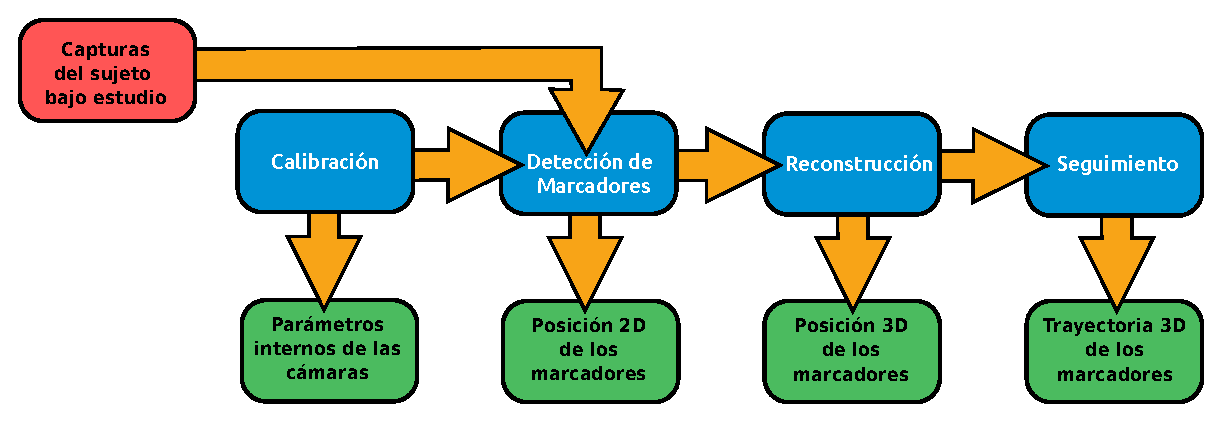
\includegraphics[scale=0.8]{img/Sistema_completo/Diagrama_de_bloques}
\end{center}
\caption{Diagrama de bloques del sistema completo.}
\label{bloquesSist}
\end{figure}


